\section{性能测试}
\subsection{使用OpenSSL测试SM4算法性能}
我们可以用openssl来测试sm4算法性能，openssl是一个开源的加密库，提供了多种加密算法的实现，包括sm4。
可以通过以下命令安装：
\begin{lstlisting}[style=Bash]
brew update
brew install openssl@3
\end{lstlisting}
安装完成后，我们可以使用以下命令来测试sm4算法的性能：
\begin{lstlisting}[style=Bash]
    openssl speed -elapsed -evp SM4-CBC
\end{lstlisting}
该命令会测试sm4算法在CBC模式下的性能，并输出吞吐量。测试结果如下：
\begin{figure}[H]
    \centering
    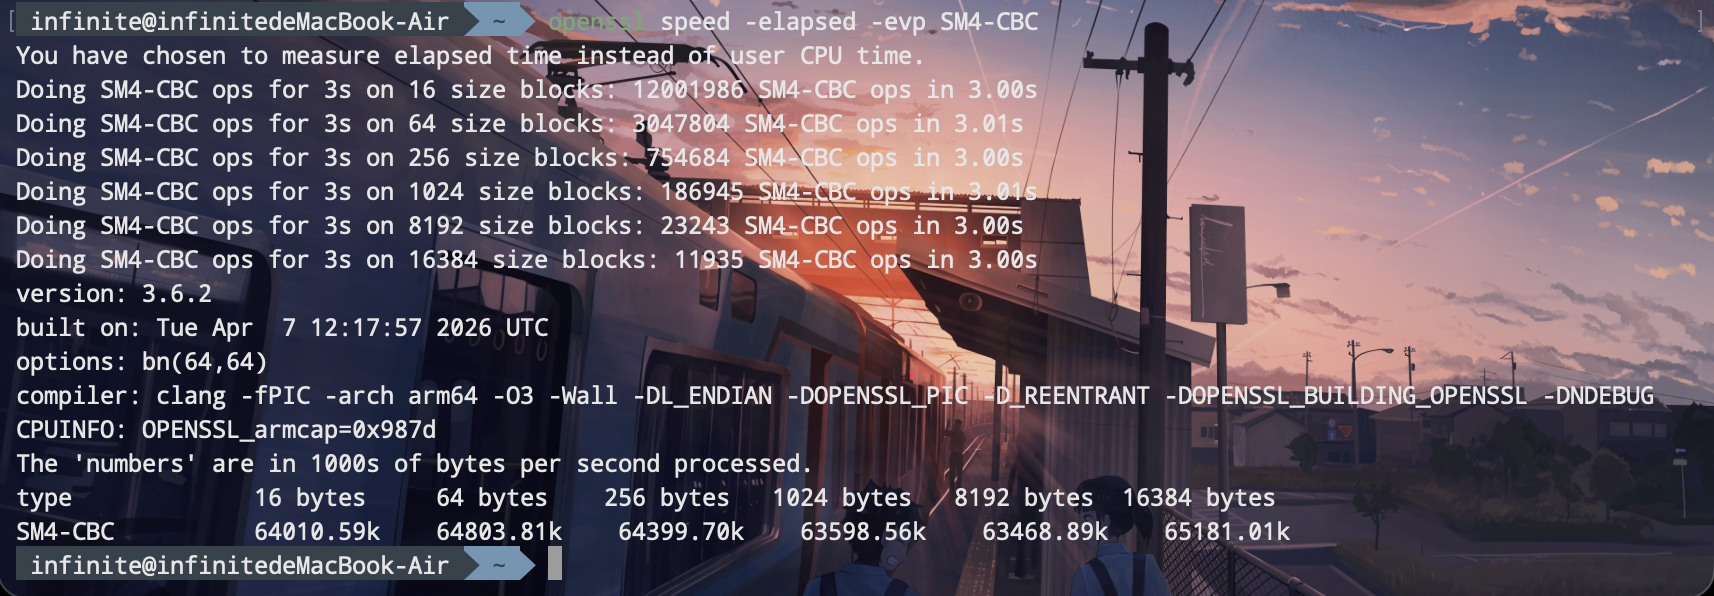
\includegraphics[width=\textwidth]{figure/openssltest.png}
    \caption{SM4-CBC性能测试结果}
    \label{fig:openssltest}
\end{figure}
OpenSSL 的 \texttt{speed} 工具并不是通过读取文件来测试算法性能，而是在内存中准备不同大小的缓冲区，然后在固定时间内反复调用 EVP 加密接口。对于每一种缓冲区大小，工具会统计在测试时间内完成的加密操作次数，并根据
\[
\text{吞吐率}
=
\frac{\text{操作次数}\times \text{缓冲区大小}}{\text{测试时间}}
\]
计算每秒处理的数据量。
例如，对于 16 字节缓冲区，测试输出为：
\begin{lstlisting}
Doing SM4-CBC ops for 3s on 16 size blocks:
12001986 SM4-CBC ops in 3.00s
\end{lstlisting}
因此其吞吐率为
\[
\frac{12001986 \times 16}{3.00}
=
64010592\ \text{bytes/s}
\]
即
\[
64010.59\ \text{kbytes/s}
\]
这与 OpenSSL 输出中的 \texttt{64010.59k} 一致。
从测试结果可以看出，sm4算法在CBC模式下的吞吐量为64MB/s\footnote{此处1MB=1000KB}左右
\subsection{未优化的SM4算法性能测试}
我们接着测试未优化的SM4算法性能。代码见附录\verb|sm4_original.c|,该版本保留逐字节S盒查表、循环移位和异或操作,作为后续查表优化与并行优化的基线。
实验分为主机环境与QEMU模拟的RISC-V环境两类:主机环境用于观察算法级优化在原生执行条件下的效果,QEMU环境用于验证同一套代码在目标RISC-V软件栈中的可移植性和性能趋势。
\subsubsection{MacBook M4测试结果}
测试环境为MacBook M4,用gcc编译,编译命令如下：
\begin{lstlisting}[style=Bash]
    gcc -std=c11 -O0 sm4_original.c -o sm4
\end{lstlisting}
编译完成后，运行测试程序，得到以下输出：
\begin{figure}[H]
    \centering
    
\includegraphics[width=\textwidth]{figure/original.png}
    \caption{未优化的SM4算法性能测试结果}
    \label{fig:sm4test}
\end{figure}
从测试结果可以看出，早期单块循环测试中未优化SM4算法的最好吞吐量为47.96MB/s,低于OpenSSL实现。后续统一数据采集脚本将数据规模扩大到1MiB并重复多轮测试,以降低计时误差和线程启动开销对结果的影响。
\subsubsection{qemu模拟riscv64架构测试结果}
在riscv64架构上,分别编译
\begin{lstlisting}[style=Bash]
    riscv64-unknown-linux-gnu-gcc -static -pthread -o sm4_original sm4_original.c
    riscv64-unknown-linux-gnu-gcc -O0 -static sm4_original.c -o sm4_original_O0
    riscv64-unknown-linux-gnu-gcc -O1 -static sm4_original.c -o sm4_original_O1
    riscv64-unknown-linux-gnu-gcc -O2 -static sm4_original.c -o sm4_original_O2
    riscv64-unknown-linux-gnu-gcc -O3 -static sm4_original.c -o sm4_original_O3
\end{lstlisting}
然后挂载
\begin{lstlisting}[style=Bash]
    mount -o loop rootfs.img  rootfs
\end{lstlisting}
复制
\begin{lstlisting}[style=Bash]
    cp -r ~/riscv64-linux/sm4_original  ~/riscv64-linux/rootfs/tmp
    cp -r ~/riscv64-linux/sm4_original_O0  ~/riscv64-linux/rootfs/tmp
    cp -r ~/riscv64-linux/sm4_original_O1  ~/riscv64-linux/rootfs/tmp
    cp -r ~/riscv64-linux/sm4_original_O2  ~/riscv64-linux/rootfs/tmp
    cp -r ~/riscv64-linux/sm4_original_O3  ~/riscv64-linux/rootfs/tmp
\end{lstlisting}
测试结果如下：
\begin{figure}[H]
    \centering
    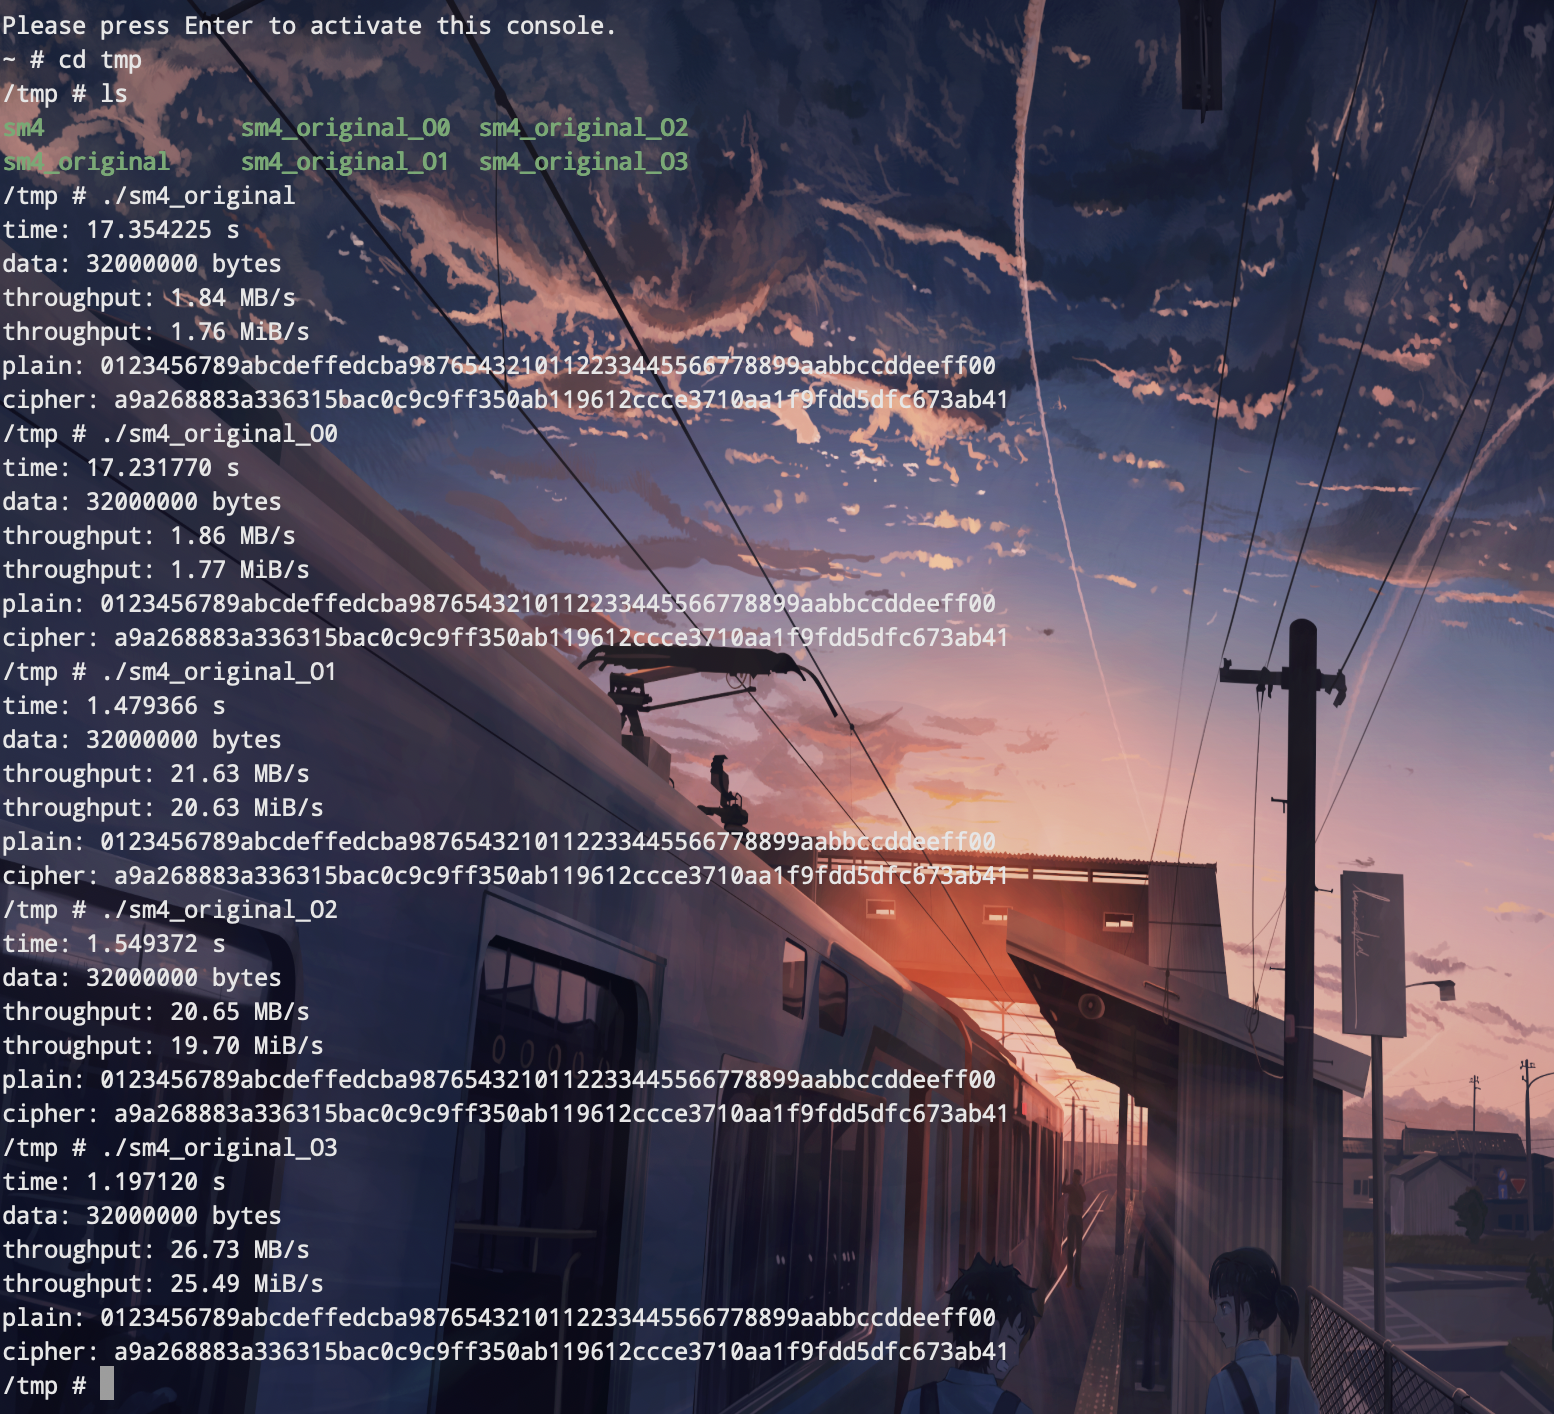
\includegraphics[width=\textwidth]{figure/riscv_original.png}
    \caption{未优化的SM4算法在riscv64架构上的性能测试结果}
    \label{fig:sm4test_riscv_default}
\end{figure}

从测试结果可以看出，未优化的SM4算法在RISC-V模拟环境中的绝对吞吐量明显低于主机原生环境,主要原因是QEMU需要进行RISC-V指令解释或动态翻译。随着编译优化级别提升,未优化版本在RISC-V环境中的吞吐量有明显提高,说明编译器优化对精简指令集平台上的循环、内联和寄存器分配尤其关键。后续实验结果章节将以CSV汇总表和统计图为主,终端截图仅作为运行过程证明。
